\section{Ba đường Conic}

%%%%%%%%%%%%%%%%%%%%%%%%%%%%%%%%%%%%%%%%%%%%%%%%%%%%%%%%%%%%%%
\subsection{Đề 1}
\Opensolutionfile{ans}[ans/ans-0-C7B4.D1]
\caulc
%Câu1
\begin{ex}%[0H9N5-1]
	Cho elip $(E)$ có phương trình chính tắc là $\dfrac{x^2}{3^2}+\dfrac{y^2}{2^2}=1$. Tìm độ dài trục lớn của $(E)$.
	\choice
	{$ 4 $}
	{\True $ 6 $}
	{$ 5 $}
	{$ 9 $}	
	\loigiai
	{
		Ta có $ a=3 $, $ b=2 $ suy ra độ dài trục lớn $ 2a=6 $.
	}
\end{ex}

%Câu2
\begin{ex}%[0H9N5-1]
	Cho elip $(E)\colon  \dfrac{x^2}{9}+\dfrac{y^2}{4}=1$. Tìm khẳng định \textbf{sai} trong các khẳng định sau.
	\choice
	{$(E)$ có tiêu điểm $F_1(-\sqrt{5} ; 0), F_2(\sqrt{5} ; 0)$}
	{$(E)$ có tỉ số $\dfrac{c}{a}=\dfrac{\sqrt{5}}{3}$}
	{$(E)$ có đỉnh $A_1(-3 ; 0)$}
	{\True $(E)$ có độ dài trục lớn là $ 3 $}
	\loigiai
	{
		Ta có $ a=3 $, $ b=2 $. Do đó $ c=\sqrt{9-4}=\sqrt{5} $.\\
		Do đó $(E)$ có tiêu điểm $F_1(-\sqrt{5} ; 0)$, $F_2(\sqrt{5} ; 0)$.\\
		Tỉ số $ \dfrac{c}{a}=\dfrac{\sqrt{5}}{3} $.\\
		$(E)$ có đỉnh $A_1(-3 ; 0)$.\\
		$(E)$ có độ dài trục lớn là $ 2a=6 $.
	}
\end{ex}

%Câu 3
\begin{ex}%[0H9N5-2]
	Cho elip $(E)$ đi qua $2$ điểm $A_1(-3;0)$, $B_1(0;-2)$. Phương trình nào là phương trình chính tắc của $(E)$?
	\choice
	{$\dfrac{x^2}{4}+\dfrac{y^2}{9}=1$}
	{\True $\dfrac{x^2}{9}+\dfrac{y^2}{4}=1$}
	{$\dfrac{x^2}{9}-\dfrac{y^2}{4}=1$}
	{$\dfrac{x^2}{4}-\dfrac{y^2}{9}=1$}
	\loigiai{
		Giả sử phương trình $(E)\colon \dfrac{x^2}{a^2}+\dfrac{y^2}{b^2}=1$, với $a,\, b>0$. \\
		Vì $(E)$ đi qua hai điểm $A_1(-3;0)$, $B_1(0;-2)$ nên ta có $a^2=9$, $b^2=2$. \\
		Vậy $(E)\colon \dfrac{x^2}{9}+\dfrac{y^2}{4}=1$.
	}
\end{ex}


%Câu4
\begin{ex}%[0H9H5-1]
	Cho elip $(E)$ có phương trình chính tắc $\dfrac{x^2}{9}+\dfrac{y^2}{4}=1$. Tổng khoảng cách từ một điểm $M$ bất kỳ trên $(E)$ đến hai tiêu điểm là 
	\choice
	{\True $6$}
	{$4$}
	{$3$}
	{$9$}
	\loigiai{
		Phương trình $(E)$ có dạng $ \dfrac{x^2}{a^2}+\dfrac{y^2}{b^2}=1$, với $a,\, b>0$, $a=3$. \\
		Theo định nghĩa $M\in (E)\Leftrightarrow MF_1+MF_2=2a=6$.\\
		Tổng khoảng cách từ một điểm $M$ bất kỳ trên $(E)$ đến hai tiêu điểm bằng $6$. 
	}
\end{ex}


%%=====Câu 5
\begin{ex}%[0H9H5-1]
	Cho elip $\left(E\right)$ có phương trình chính tắc là $\dfrac{x^2}{9}+\dfrac{y^2}{4}=1$. Gọi $A_1$, $A_2$ là các đỉnh của $(E)$ thuộc trục $Ox$. Tính độ dài đoạn thẳng $A_1A_2$.
	\choice
	{\True $A_1A_2=6$}
	{$A_1A_2=4$}
	{$A_1A_2=5$}
	{$A_1A_2=2\sqrt{5}$}
	\loigiai{
		Vì $(E)\colon\dfrac{x^2}{9}+\dfrac{y^2}{4}=1$ suy ra $A_1(-3;0)$ và $A_2(3;0)$. Mặt khác $A_1A_2=2a=6$.
	}
\end{ex}
%%=====Câu 6
\begin{ex}%[0H9H5-1]
	Cho elip $\left(E\right)$ có phương trình chính tắc là $\dfrac{x^2}{25}+\dfrac{y^2}{16}=1$. Tính tổng độ dài các trục của $(E)$.
	\choice
	{\True $10$}
	{$9$}
	{\True $18$}
	{$8$}
	\loigiai{
		Từ phương trình của elip ta suy ra trục lớn là $2a=10$, trục bé $2b=8$. Tổng độ dài hai trục là $18$.
	}
\end{ex}



%%=====Câu 7
\begin{ex}%%[0H9N5-1]
	Cho elip $(E)$ có phương trình chính tắc là $\dfrac{x^2}{5}+\dfrac{y^2}{1}=1$. Tìm toạ độ các tiêu điểm của $(E)$. 
	\choice
	{ $F_1(-1;0)$ và $F_2(1;0)$}
	{\True $F_1(-2;0)$ và $F_2(2;0)$}
	{$F_1(2;0)$ và $F_2(-2;0)$}
	{$F_1(\sqrt{5};0)$ và $F_2(-\sqrt{5};0)$}
	\loigiai{Ta có $a=\sqrt{5}$, $b=1$, suy ra $c=2$ do đó  $F_1(-2;0)$ và $F_2(2;0)$.
	}
\end{ex}

%Câu 8
\begin{ex}%[0H9H5-2]
	Cho elip $(E)$ có  độ dài trục lớn là $6$, độ dài tiêu cự  là $4$. Lập phương trình chính tắc của $(E)$.
	\choice
	{ \True $\dfrac{x^2}{9}+\dfrac{y^2}{5}=1$}
	{$\dfrac{x^2}{36}+\dfrac{y^2}{16}=1$}
	{ $\dfrac{x^2}{5}+\dfrac{y^2}{9}=1$}
	{$\dfrac{x^2}{9}-\dfrac{y^2}{5}=1$}
	\loigiai{
		Ta có $\heva{&2a=6\\& 2c=4}\Leftrightarrow \heva{&a=3\\&c=2}\Rightarrow b^2=a^2-c^2=5$, do đó do đó phương trình chính tắc của $(E)$ là $\dfrac{x^2}{9}+\dfrac{y^2}{5}=1$.
	}
\end{ex}


%%=====Câu 9
\begin{ex}%%[0H9H5-1]
	Cho elip $(E)$ có phương trình chính tắc là $\dfrac{x^2}{25}+\dfrac{y^2}{16}=1$. Tính tính diện tích hình chữ nhật đi qua 4 đỉnh của $(E)$.
	\choice
	{ $20$}
	{\True $80$}
	{$48$}
	{$60$}
	\loigiai{Ta có $a=5$, $b=4$, do đó  diện tích hình chữ nhật đi qua 4 đỉnh của $(E)$ là $2b\cdot 2a=80$.
	}
\end{ex}

%%=====Câu 10
\begin{ex}%%[0H9H5-3]
	Cho elip $(E)$ có phương trình $\dfrac{x^2}{25}+\dfrac{y^2}{9}=1$. Đường thẳng $(d)\colon x=-4$ cắt $(E)$ tại hai điểm $M$, $N$. Khi đó 
	\choice
	{ $MN=\dfrac{9}{25}$}
	{$MN=\dfrac{18}{25}$}
	{\True $MN=\dfrac{18}{5}$}
	{$MN=\dfrac{9}{5}$}
	\loigiai{$M(x;y)$ nằm trên $(d)$ nên $x=-4$, suy ra
		$$\dfrac{(-4)^2}{25}+\dfrac{y^2}{9}=1\Leftrightarrow \dfrac{y^2}{9}=\dfrac{9}{25}\Leftrightarrow y^2=\dfrac{81}{25}\Leftrightarrow\hoac{& y=-\dfrac{9}{5}\\& y=\dfrac{9}{5}.}$$
		Vậy $M\left(-4;- \dfrac{9}{5}\right)$ và $N\left(-4; \dfrac{9}{5}\right)$. Do đó $MN=\sqrt{(-4+4)^2 +\left( \dfrac{9}{5}+\dfrac{9}{5}\right)^2}=\dfrac{18}{5}$.
	}
\end{ex}

%%=====Câu 11
\begin{ex}%%[0H9H5-2]
	Cho elip $(E)$ có một đỉnh $A_1(-4;0)$, một tiêu điểm $F_2(3;0)$.  Lập phương trình chính tắc của $(E)$.
	\choice
	{ \True $\dfrac{x^2}{16}+\dfrac{y^2}{7}=1$}
	{$\dfrac{x^2}{16}+\dfrac{y^2}{9}=1$}
	{ $\dfrac{x^2}{9}+\dfrac{y^2}{7}=1$}
	{$\dfrac{x^2}{16}-\dfrac{y^2}{5}=1$}
	\loigiai{Ta có đỉnh $A_1(-4;0)$, một tiêu điểm $F_2(3;0)$, suy ra $a=4$,  $c=3$ và $b^2=a^2-c^2=7$, do đó  $\dfrac{x^2}{16}+\dfrac{y^2}{7}=1$.
	}
\end{ex}
%%=====Câu 12
\begin{ex}%[0H9H5-2]
	Cho elip $(E)$ đi qua một điểm $M(-3\sqrt{2};\dfrac{3\sqrt{2}}{2})$, một tiêu điểm $F_1(-3\sqrt{3};0)$.  Lập phương trình chính tắc của $(E)$.
	\choice
	{ \True $\dfrac{x^2}{36}+\dfrac{y^2}{9}=1$}
	{$\dfrac{x^2}{25}+\dfrac{y^2}{9}=1$}
	{ $\dfrac{x^2}{36}+\dfrac{y^2}{25}=1$}
	{$\dfrac{x^2}{36}-\dfrac{y^2}{9}=1$}
	\loigiai{Ta có một tiêu điểm $F_1(-3\sqrt{3};0)$, suy ra  $c=3\sqrt{3}$ và $a^2-b^2=27$.\\
		Vì $M \in (E)$ nên $\dfrac{18}{a^2}+\dfrac{9}{2b^2}=1$. Ta có hệ phương trình $\heva{&a^2-b^2=36\\&\dfrac{x^2}{a^2}+\dfrac{y^2}{b^2}=1} \Leftrightarrow \heva{&a^2=36 \\&b^2=9.}$\\
		Do đó  phương trình chính tắc của $(E)$ là $\dfrac{x^2}{36}+\dfrac{y^2}{9}=1$.
	}
\end{ex}


\Closesolutionfile{ans}
\indapan{6}{ans/ans-0-C7B4.D1}

%%%%%%%%%%%%%%%%%%%%%%%%%%%%%%%%%%%%%%%%%%%%%%%%%%%%%%%%%%%%%%%%%%%%%%%%%%%%%%%%%%%%%%%%%%%%%%%%%%%
\cauds
\Opensolutionfile{ans}[ans/ans-0-C7B4.D1-DS]
\begin{ex}%%[0H9H5-7]
	Cho parabol $(P)$ có dạng $y=2px$ ($p>0$), đi qua điểm $A\left( \dfrac{3}{4};-9\right)$. Khi đó các khẳng định sau đúng hay sai?
	\choiceTF
	{$x=54$ là phương trình đường chuẩn của parabol $(P)$}
	{\True Parabol $(P)$ đi qua điểm $B(1;6\sqrt{3})$}
	{\True Parabol $(P)$ đi qua điểm $C(1;-6\sqrt{3})$}
	{\True  Parabol $(P)$ cắt đường thẳng $y=x+1$ tại hai điểm}
	\loigiai{
		Gọi phương trình parabol $(P)$ có dạng $y=2px$ ($p>0$).\\
		Có $A\left( \dfrac{3}{4};-9\right)\in (P) $ nên $(-9)^2=2\cdot p\cdot \dfrac{3}{4}\Leftrightarrow 2p=108$.\\
		Vậy parabol $(P)\colon y^2=108 x$.
		\begin{itemchoice}
			\itemch Sai.
			$x=-\dfrac{p}{2}\Leftrightarrow x=-27$ là phương trình đường chuẩn của parabol $(P)$.
			\itemch Đúng.
			Parabol $(P)$ đi qua điểm $B(1;6\sqrt{3})$.
			\itemch Đúng.
			Parabol $(P)$ đi qua điểm $C(1;-6\sqrt{3})$.
			\itemch Đúng. Tọa độ giao điểm của parabol $(P)$ và đường thẳng $y=x+1$ là nghiệm của hệ phương trình $\heva{&y^2=108x\\&y=x+1}\Leftrightarrow \heva{&y=x+1\\&(x+1)^2=108x}\Leftrightarrow \heva{&y=x+1\\&x^2-106x+1=0. \ (*)}$ 
			Phương trình $(*)$ có hai nghiệm phân biệt ($\Delta>0$) nên parabol $(P)$ cắt đường thẳng $y=x+1$ tại hai điểm. 
		\end{itemchoice}
	}
\end{ex}
%% Câu 2
\begin{ex}%[0H9H5-0]
	Xác định tính đúng sai của các khẳng định sau?
	\choiceTF
	{$\dfrac{x^2}{5}+\dfrac{y^2}{4}$ có tiêu cự bằng $1$}
	{\True $\dfrac{x^2}{7}-\dfrac{y^2}{10}$ có hai tiêu điểm là $F_1(-\sqrt{17};0)$, $F_2(\sqrt{17};0)$}
	{\True $y^2=18x$ có đường chuẩn $x+\dfrac{9}{2}=0$}
	{\True$y^2=18x$ có tiêu điểm $F\left( \dfrac{9}{2};0\right)$}
	\loigiai{
		\begin{itemchoice}
			\itemch Sai.\\
			$\dfrac{x^2}{5}+\dfrac{y^2}{4}$  là phương trình chính tắc của đường elip với $\heva{&a=\sqrt{5}\\& b=2}\Rightarrow c^2=a^2-b^2=1$. Do đó tiêu cự $2c=2$.
			\itemch Đúng.\\
			$\dfrac{x^2}{7}-\dfrac{y^2}{10}$ là phương trình chính tắc của hypebol với $\heva{&a=7\\&b=\sqrt{10}.}$\\
			Suy ra $c^2=a^2+b^2=17\Rightarrow c=\sqrt{17}$.\\
			 Do đó hai tiêu điểm là $F_1(-\sqrt{17};0)$, $F_2(\sqrt{17};0)$.
			\itemch Đúng.\\
			$y^2=18x$ là phương trình chính tắc của parabol với $p=9$. Vậy đường chuẩn là $x+\dfrac{9}{2}=0$.
			\itemch Đúng.\\
			$y^2=18x$ là phương trình chính tắc của parabol với $p=9$. Vậy tiêu điểm $F\left( \dfrac{9}{2};0\right)$.
		\end{itemchoice}
	}
\end{ex}


%% Câu 3
\begin{ex}%[0H9H5-7]
	Cho hypebol có phương trình $16x^2-9y^2=144$ $(P)$. Khi đó, các khẳng định sau đúng hay sai?
	\choiceTF
	{Tiêu điểm của $(H)$ là $F_1(-4;0)$; $F_2(4;0)$}
	{\True Tiêu cự bằng $10$}
	{\True Có hai điểm thuộc  $(H)$ có hoành độ $x=9$}
	{  Khi $-4<k<4$ thì đường thẳng $(d)\colon y=kx$ có điểm chung với hypebol trên}
	\loigiai{
		\begin{itemchoice}
			\itemch Sai. Ta có $(H)\colon 16x^2-9y^2=144\Leftrightarrow \dfrac{x^2}{9}-\dfrac{y^2}{16}=1$.\\
			 Do đó $\heva{&a=3\\&b=4}$ nên $c=\sqrt{a^2+b^2}=5$. Tiêu điểm của $(H)$ là $F_1(-4;0)$; $F_2(4;0)$.	
			\itemch Đúng. Tiêu cự $F_1F_2=2c=10$.		
			\itemch Đúng. Thay $x=9$ vào $(H)\colon  \dfrac{x^2}{9}-\dfrac{y^2}{16}=1$ ta có $\dfrac{y^2}{16}=8\Leftrightarrow y^2=128\Leftrightarrow y=\pm 8\sqrt{2}$. Vậy có hai điểm thuộc  $(H)$ có hoành độ $x=9$ là $M_1(9;-8\sqrt{2})$; $M_2(9; 8\sqrt{2})$.		
			\itemch Sai. Tọa độ giao điểm của hypebol $(H)$ và đường thẳng $(d)$ là nghiệm của hệ $\heva{&16x^2-9y^2=144\\&y=kx}\Rightarrow 16x^2-9k^2x^2=144\Leftrightarrow (16-9k^2)x^2=144\ (*)$.\\
			Đường thẳng $(d)$ cắt $(H)\Leftrightarrow  (*)$ có nghiệm $\Leftrightarrow 16-9k^2>0\Leftrightarrow -\dfrac{4}{3}<k<\dfrac{4}{3}$.
	\end{itemchoice}}
\end{ex}


%%Câu 4
\begin{ex}%[0H9V5-7]
	Trong mặt phẳng $Oxy$, cho parabol $(P)\colon y^2=8x$. Khi đó, các khẳng định sau là đúng hay sai?
	\choiceTF
	{\True Tiêu điểm $F(2;0)$}
	{\True Có hai điểm $M$ trên $(P)$, cách $F$ một khoảng là $3$}
	{Điểm $M$ trên $(P)$ sao cho $S_{\triangle OMF}=8$, có hoành độ bằng $6$}
	{Tồn tại điểm $A$ nằm trên parabol và điểm $B$ nằm trên đường thẳng $(\Delta)\colon 4x-3y+5=0$ sao cho đoạn thẳng $AB$ ngắn nhất, khi đó $AB$ ngắn nhất bằng $\dfrac{1}{5}$}
	\loigiai{
		\begin{center}	
			\begin{tikzpicture}[scale=0.4, font=\footnotesize, line join=round, line cap=round, >=stealth]
				\def\xmin{-3}\def\xmax{5}\def\ymin{-4}\def\ymax{4}\pgfmathsetmacro\p{2}
				\draw[->] (\xmin-0.2,0)--(\xmax+0.2,0) node[below] {\footnotesize $x$};
				\draw[->] (0,\ymin-0.2)--(0,\ymax+0.2) node[right] {$y$};
				\clip (\xmin,\ymin) rectangle (\xmax,\ymax);
				\path
				(0,0)coordinate (O)
				(-\p,0) coordinate (H)node[above left ]{$\frac{-p}{2}$}
				(\p,0) coordinate (F)node[above right]{$\frac{p}{2}$}
				(1,2) coordinate (M)
				(-\p,2)coordinate (N)
				;
				\draw
				(N)--(M)--(F)
				(-\p,\ymin)--(-\p,\ymax);
				\draw[smooth,variable=\x,blue] plot ({0.25*\x*\x},{\x});
				\fill (M)node[right]{$M$} circle (1.5pt);
				\foreach \x/\g in {H/-130,F/-90,O/-120}
				\fill (\x) circle (1.5pt) ($(\x)+(\g:5mm)$) node{$\x$};
			\end{tikzpicture}
		\end{center}
		\begin{itemchoice}
			\itemch	Đúng. Từ phương trình của $(P)$ suy ra $p=4$ nên tiêu điểm $F(2;0)$.
			\itemch	Đúng. Giả sử $M(x_M; y_M)\in (P)$ suy ra $y_M^2=8x_M$. Ta có $3=FM=x_M+\dfrac{p}{2}$ suy ra $x_M=1$, thay vào $y_M^2=8x_M\Rightarrow y_M=\pm 2\sqrt{2}$.\\
			Vậy có hai điểm thỏa mãn là $M_1(1;2\sqrt{2})$, $M_2(1;-2\sqrt{2})$.
			\itemch Sai. Ta có $M\in (P)$ nên $M\left(\dfrac{a^2}{8}; a\right)$ với $a\ge 0$. Suy ra $\mathrm{d}(M;OF)=y_M=a$.
			$$S_{\triangle OFM}=8\Leftrightarrow \dfrac{1}{2}OF\cdot \mathrm{d}(M;OF)=8\Leftrightarrow a=8.$$
			Vậy điểm cần tìm là $M(8;8)$.
			\itemch	Sai. Với mọi điểm $A\in (P)$, $B\in (\Delta)$, ta luôn có $AB\ge \mathrm{d}(A;\Delta)$.\\
			$A\in (P)\Rightarrow A\left( \dfrac{a^2}{8};a\right)$ với $a\ge 0$. Khi đó, $$\mathrm{d}(A;\Delta)=\dfrac{\left|4\cdot \frac{a^2}{8} -3\cdot a+5 \right|}{5}=\dfrac{(a-3)^2+1}{10}\ge \dfrac{1}{10}.$$
			Suy ra $\mathrm{d}(A;\Delta)$ ngắn nhất khi $a=3$; $A\left( \dfrac{9}{8};3\right)$ và $B$ là hình chiếu của $A$ lên $(\Delta)$.\\
			Đường thẳng đi qua $A$ vuông góc với $(\Delta)$ nhận $\vec{u}(3;4)$ làm véc-tơ pháp tuyến nên có phương trình 
			$$3\left(x-\dfrac{9}{8}\right)+4(y-3)=0\Leftrightarrow 24x+32y-123=0.$$
			Do đó tọa độ điểm $B$ là nghiệm của hệ $\heva{& 4x-3y+5=0\\&24x+32y-123=0}\Leftrightarrow \heva{&x=\dfrac{209}{200}\\&y=\dfrac{153}{50}.}$\\
			Vậy có $A\left( \dfrac{9}{8};3\right)$, $B\left( \dfrac{209}{200};\dfrac{153}{50}\right)$ để $AB$ ngắn nhất và $AB$ ngắn nhất bằng $\dfrac{1}{10}$.
		\end{itemchoice}
	}
\end{ex}
\Closesolutionfile{ans}
\indapan{3}{ans/ans-0-C7B4.D1-DS}
%%%%%%%%%%%%%%%%%%%%%%%%%%%%%%%%%%%%%%%%%%%%%%%%%%%%%%%%%%%%%
\Opensolutionfile{ans}[ans/ans-0-C7B4.D1-KQ]
\caukq
%%Câu 1
\begin{ex}%%[0H9H5-3]
	Trong mặt phẳng tọa độ $Oxy$, cho điểm $M$ chuyển động trên elip $(E)\colon \dfrac{x^2}{25}+\dfrac{y^2}{16}=1$ và điểm $D(6;0)$. Gọi $a$ và $b$ lần lượt là giá trị nhỏ nhất và giá trị lớn nhất của $DM$. Khi đó $T=2a+b$ bằng?
	\shortans{$13$}
	\loigiai{
		\begin{center}
			\begin{tikzpicture}[scale=1, font=\footnotesize, line join=round, line cap=round, >=stealth]
				\def\xmin{-3.5}\def\xmax{3.5}\def\ymin{-2.5}\def\ymax{2.5}\pgfmathsetmacro\c{1.5}
				\draw[->] (\xmin-0.2,0)--(\xmax+0.2,0) node[below] {\footnotesize $x$};
				\draw[->] (0,\ymin-0.2)--(0,\ymax+0.2) node[right] {$y$};
				\draw (0,0) node [below left] {$O$};
				\clip (\xmin,\ymin) rectangle (\xmax,\ymax);
				\path
				(-2.5,0) coordinate (A_1)node[below left]{$-5$}
				(2.5,0) coordinate (A_2)node[below left]{$5$}
				(0,-2) coordinate (B_1)node[below left]{$-4$}
				(0,2) coordinate (B_2)node[above left]{$4$}
				(3,0) coordinate (D)node[below]{$6$}
				(-\c,0) coordinate (F_1)node[above]{$-3$}
				(\c,0) coordinate (F_2)node[above left]{$3$}
				(1.5,1.6) coordinate (M)
				;
				\draw [blue]
				(0,0)  ellipse (2.5cm and 2cm);
				\draw
				(F_1)--(M)--(F_2)--cycle (D)--(M)
				;
				\fill (M)node[above]{$M$} circle (1.5pt);
				\foreach \x/\g in {D/40,F_1/-90,F_2/-90}
				\fill (\x) circle (1.5pt) ($(\x)+(\g:3mm)$) node{$\x$};
			\end{tikzpicture}
		\end{center}
		Ta có $\heva{&DO-OM\le DM\le DO+OM\\& OM\le 5\\& DO=6}\Rightarrow 6-5\le DM\le 6+5\Rightarrow 1\le DM\le 11$.\\
		Vậy $DM$ đạt giá trị nhỏ nhất là $a=1$ và đạt giá trị lớn nhất là $b=11$, do đó $T=2a+b=13$.
	}
\end{ex}
%%Câu 2
\begin{ex}%%[0H9H5-8]
	Cho parabol $(P)\colon y^2=2px$ ($p>0$). Biết $(P)$ có  đường chuẩn $\Delta$ song song và cách đường thẳng $d\colon x=2$ một khoảng bằng $5$. Khi đó giá trị của $p$ bằng bao nhiêu?
	\shortans{$6$}
	\loigiai{
		Vì $(P)$ có phương trình chính tắc là $y^2=2px$ ($p>0$) nên phương trình đường chuẩn $\Delta$ có dạng $x=-\dfrac{p}{2}$. Theo giả thiết
		$$\mathrm{d}(d,\Delta)=5\Rightarrow \left|\dfrac{-p}{2}-2 \right|=5\Leftrightarrow\hoac{& \dfrac{-p}{2}-2=5\\&\dfrac{-p}{2}-2=-5 } \Leftrightarrow \hoac{&p=-14<0 \text{ (loại)}\\& p=6>0.}$$
		Vậy $p=6$.	
	}
\end{ex}
%%Câu 3
\begin{ex}%%[0H9V5-9]
	Cho phương trình chính tắc của elip $(E)\colon \dfrac{x^2}{a^2}+\dfrac{y^2}{b^2}=1$ ($a>b>0$). Biết $(E)$ đi qua điểm $M(2\sqrt{2};2)$ và $M$ nhìn hai tiêu điểm của elip dưới một góc vuông. Khi đó $T=a^2+2b^2$ bằng bao nhiêu?
	\shortans{$40$}
	\loigiai{
		\begin{center}
			\begin{tikzpicture}[scale=1, font=\footnotesize, line join=round, line cap=round, >=stealth]
				\def\xmin{-3}\def\xmax{3}
				\def\ymin{-2}\def\ymax{2}
				\pgfmathsetmacro\c{2}
				\draw[->] (\xmin-0.2,0)--(\xmax+0.2,0) node[below] {\footnotesize $x$};
				\draw[->] (0,\ymin-0.2)--(0,\ymax+0.2) node[right] {$y$};
				\draw (0,0) node [below left] {$O$};
				\clip (\xmin,\ymin) rectangle (\xmax,\ymax);
				\path
				(-\c,0) coordinate (F_1)
				(\c,0) coordinate (F_2)
				(1.43,1.1) coordinate (M)
				;
				\draw [blue]
				(0,0)  ellipse (2.43cm and 1.4cm);
				\draw
				(F_1)--(M)--(F_2)--cycle
				;
				\fill (M)node[above]{$M$} circle (1.5pt);
				\foreach \x/\g in {F_1/-90,F_2/-90}
				\fill (\x) circle (1.5pt) ($(\x)+(\g:3mm)$) node{$\x$};
				\draw pic[draw,angle radius=2mm]{right angle=F_1--M--F_2};
			\end{tikzpicture}
		\end{center}
		Phương trình chính tắc của elip $(E)\colon \dfrac{x^2}{a^2}+\dfrac{y^2}{b^2}=1$ ($a>b>0$). \\
		Gọi hai tiêu điểm của $(E)$ là $F_1(-c;0)$, $F_2(c;0)$. Khi đó, $\heva{&\overrightarrow{MF_1}=(-c-2\sqrt{3};-2)\\&\overrightarrow{MF_2}=(c-2\sqrt{3};-2).}$\\
		Ta có $MF_1\perp MF_2\Leftrightarrow \overrightarrow{MF_1}\cdot \overrightarrow{MF_2}=0\Leftrightarrow (-c-2\sqrt{3})(c-2\sqrt{3})+4=0\Leftrightarrow c^2=16$.\\
		Suy ra $a^2-b^2=16\Rightarrow a^2=16+b^2$.\\
		Lại có $(E)$ đi qua $M(2\sqrt{3};3)$ nên $$\dfrac{12}{a^2}+\dfrac{4}{b^2}=1\Leftrightarrow \dfrac{12}{b^2+16}+\dfrac{4}{b^2}=1\Leftrightarrow 12b^2+4b^2+64=b^4+16b^2\Leftrightarrow b^4=64\Leftrightarrow b^2=8.$$
		 Vậy $\heva{&a^2=24\\&b^2=8}$ và $T=a^2+2b^2=40$.	
	}
\end{ex}
%%Câu 4
\begin{ex}%%[0H9V5-9]
	Cho parabol $(P)\colon y^2=16x$ và đường thẳng $(d)\colon x=a$ ($a>0$). Tìm $a$ để $(d)$ cắt $(P)$ tại hai điểm phân biệt $A$ và $B$ sao cho $\widehat{AOB}=120^\circ$.
	\shortans{$5{,}33$}
	\loigiai{
		\begin{center}	
			\begin{tikzpicture}[scale=0.8, font=\footnotesize, line join=round, line cap=round, >=stealth]
				\def\xmin{-1}\def\xmax{3.4}\def\ymin{-3}\def\ymax{3}\pgfmathsetmacro\p{2}
				\draw[->] (\xmin-0.2,0)--(\xmax+0.2,0) node[below] {\footnotesize $x$};
				\draw[->] (0,\ymin-0.2)--(0,\ymax+0.2) node[right] {$y$};
				\clip (\xmin,\ymin) rectangle (\xmax,\ymax);
				\path
				(0,0)coordinate (O)
				(1,2) coordinate (A)
				(1,-2) coordinate (B)
				;
				\draw
				(A)--(O)--(B)
				(1,\ymin)--(1,\ymax);
				\draw[smooth,variable=\x,blue] plot ({0.25*\x*\x},{\x});
				\foreach \x/\g in {A/-30,B/30,O/-120}
				\fill (\x) circle (1.5pt) ($(\x)+(\g:5mm)$) node{$\x$};
			\end{tikzpicture}
		\end{center}
		Tọa độ giao điểm của $(d)$ và $(P)$ là $\heva{&x=a\\&y^2=16x}\Leftrightarrow\heva{&x=a\\&y^2=16a}\Leftrightarrow \heva{&x=a\\&y=\pm 4\sqrt{a}.}$\\
		 Vậy giao điểm của của $(d)$ và $(P)$ là $A(a;-4\sqrt{a})$, $B(a;4\sqrt{a})$.\\
		$\widehat{AOB}=120^\circ\Leftrightarrow \left(\overrightarrow{OA},\overrightarrow{OB}\right)=120^\circ\Leftrightarrow \cos\left(\overrightarrow{OA},\overrightarrow{OB}\right)=-\dfrac{1}{2}$\\
		$\Leftrightarrow \dfrac{a^2-16a}{\sqrt{a^2+16a}\cdot \sqrt{a^2+16a}}=-\dfrac{1}{2}\Leftrightarrow -2(a^2-16a)=a^2+16a\Leftrightarrow a=\dfrac{16}{3}>0$.\\
		Vậy $a\approx 5{,}33$.
	}
\end{ex}
%%Câu 5
\begin{ex}%%[0H9V5-0]
	Để chụp toàn cảnh, ta có thể sử dụng một gương hypebol. Máy ảnh được hướng về phía đỉnh của gương và tâm quang học của máy ảnh được đặt tại một tiêu điểm của gương (xem hình). Tìm khoảng cách từ tâm quang của máy ảnh đến đỉnh của gương, biết rằng phương trình mặt cắt của gương là $\dfrac{x^2}{25}-\dfrac{y^2}{16}=1$.
	\shortans{$11{,}2$}
	\begin{center}	
		\begin{tikzpicture}[scale=0.6, font=\footnotesize, line join=round, line cap=round, >=stealth]
			\def\xmin{-10}\def\xmax{10}\def\ymin{-5}\def\ymax{5}\pgfmathsetmacro\c{2*sqrt(5)}
			\draw[->] (\xmin-0.2,0)--(\xmax+0.2,0) node[below] {\footnotesize $x$};
			\draw[->] (0,\ymin-0.2)--(0,\ymax+0.2) node[right] {$y$};
			\clip (\xmin,\ymin) rectangle (\xmax,\ymax);
			\path
			(0,0)coordinate (O)
			(-2,0) coordinate (A_1)
			(2,0) coordinate (A_2)
			(-\c,0) coordinate (F_1)
			(\c,0) coordinate (F_2)
			(-6.3,3) coordinate (M)
			(-6.3,-3) coordinate (N)
			;
			\draw[blue] (M)--(N);
			\fill[blue!50] (F_2)circle (0.3cm);
			\fill[blue!10] (M)--(N)--plot ({-2*sqrt(\x*\x+1)},{\x})--(M);
			\draw[smooth,variable=\x,blue] plot ({2*sqrt(\x*\x+1)},{\x});
			\draw[smooth,variable=\x,blue] plot ({-2*sqrt(\x*\x+1)},{\x});
			\foreach \x/\g in {F_1/-90,F_2/-90}
			\fill (\x) circle (4.5pt) ;
			\foreach \x/\g in {F_1/-90,F_2/-90,A_1/-40,A_2/240,O/-120}
			\fill (\x) circle (1.5pt) ($(\x)+(\g:7mm)$) node{$\x$};
			\draw (M)--($(M)+(30:1)$)node[above]{gương hypebol};
			\draw (F_2)--($(F_2)+(130:3)$)node[above]{tâm máy ảnh};
			\draw[dashed](A_1)--(F_1);
		\end{tikzpicture}
	\end{center}
	\loigiai{ Gọi $(H)\colon \dfrac{x^2}{25}-\dfrac{y^2}{16}=1\Rightarrow \heva{&a^2=25\\&b^2=16}\Rightarrow \heva{&a=5\\&b=4}\Rightarrow c=\sqrt{a^2+b^2}=\sqrt{39}$.\\
		Tiêu điểm của gương là $F_1(-\sqrt{39};0)$ và $F_2(\sqrt{39};0)$.\\
		Đỉnh của gương là $A_1(-5;0)$.\\
		Vậy khoảng cách từ tâm của máy ảnh tới đỉnh của gương là\\ $F_2A_1=OA_1+OF_2=5+\sqrt{39}\approx 11{,}2$.		
	}
\end{ex}
%%Câu 6
\begin{ex}%[0H9V5-0]
	\immini{
	Một elip  $(E)\colon \dfrac{x^2}{a^2}+\dfrac{y^2}{b^2}=1$, ($a>b>0$) với bán trục lớn $a$, bán tiêu cự $c$, thì tỉ số $e=\dfrac{c}{a}$ được gọi là tâm sai của elip. Quỹ đạo của trái đất quay quanh mặt trời là một elip $(E)$, trong đó mặt trời là  một trong các tiêu điểm. Biết khoảng cách nhỏ nhất và lớn nhất giữa mặt trời và trái đất lần lượt là $147$ triệu km và $152$ triệu km. Tâm sai của elip $(E)$ là $\dfrac{m}{n}$ (với $\dfrac{m}{n}$ là phân số tối giản). Tính $T=m+n$.
	\shortans{$304$}}
	{	\begin{tikzpicture}[scale=1, font=\footnotesize, line join=round, line cap=round, >=stealth]
			\def\xmin{-3.5}\def\xmax{3.5}\def\ymin{-2.5}\def\ymax{2.5}\pgfmathsetmacro\c{1.5}
			\clip (\xmin,\ymin) rectangle (\xmax,\ymax);
			\path
			(-\c,0) coordinate (F_1)
			(1.5,1.6) coordinate (M)
			;
			\draw [blue]
			(0,0)  ellipse (2.5cm and 2cm);
			\fill[blue] (M)node[above right ]{Trái đất} circle (2.5pt);
			\fill[red] (F_1)  node[below]{Mặt trời} circle (5pt);
		\end{tikzpicture}}
	\loigiai{Elip có phương trình $(E)\colon \dfrac{x^2}{a^2}+\dfrac{y^2}{b^2}=1$, ($a>b>0$), $c=\sqrt{a^2-b^2}$.\\
	 Khoảng cách từ một điểm $M$ bất kỳ thuộc elip có hoành độ $x_M$ là $d_M=a\pm \dfrac{c\cdot x_M}{a}$, cho nên khoảng cách lớn nhất và nhỏ nhất từ một tiêu điểm đến $M$ lần lượt là $a+c$ và $a-c$.\\
		Ta có hệ phương trình $\heva{&a+c=152\\&a-c=147}\Leftrightarrow \heva{&a=\dfrac{299}{2}\\&c=\dfrac{5}{2}.}$\\
		Vậy tâm sai của elip $(E)$ là $e=\dfrac{c}{a}=\dfrac{5}{299}\Rightarrow \heva{&m=5\\& n=299}$ và $T=m+n=304$.
	}
\end{ex}
\Closesolutionfile{ans}
\indapan{6}{ans/ans-0-C7B4.D1-KQ}
%%%%%%%%%%%%%%%%%%%%%%%%%%%%%%%%%%%%%%%%%%%%%%%%%%%%%%%%%%%%%%%%%
\newpage
\subsection{Đề 2}
\Opensolutionfile{ans}[ans/ans-0-C7B4.D2]
\caulc
%Câu 1
\begin{ex}% %[0H9N5-1]
	Cho elip $(E)$ có phương trình chính tắc là $\dfrac{x^2}{25}+\dfrac{y^2}{16}=1$. Tìm độ dài trục bé  của $(E)$.
	\choice
	{ $10$}
	{\True $8$}
	{$9$}
	{$6$}
	\loigiai{Ta có  $b=4$, do đó  độ dài trục bé của $(E)$ là $2b=8$.
	}
\end{ex}
%Câu 2
\begin{ex}%[0H9N5-1]
	Cho elip $(E)\colon  x^2+4 y^2=1$. Tìm mệnh đề
	đúng trong các mệnh đề sau.
	\choice
	{$(E)$ có độ dài trục lớn bằng $ 4 $}
	{$ (E) $ có độ dài trục bé bằng $ 2 $}
	{\True $(E)$ có đỉnh $A_1(-1 ; 0)$}
	{$(E)$ có tiêu cự bằng $2\sqrt{3}$}
	\loigiai
	{
		Ta viết lại $ (E)\colon \dfrac{x^2}{1}+\dfrac{y^2}{\frac{1}{4}} =1$.
		Khi đó $ a=1 $, $ b=\dfrac{1}{2} $, $ c=\dfrac{\sqrt{3}}{2} $.
		\begin{itemize}
			\item $ (E) $ có độ dài trục lớn bằng $ 2 $.
			\item $ (E) $ có độ dài  trục bé bằng $ 1 $.
			\item $ (E) $ có đỉnh là $ (-1;0) $ và $ (1;0) $.
			\item$ (E) $ có tiêu cự $ \sqrt{3} $.
		\end{itemize}
	}
\end{ex}

%Câu 3
\begin{ex}%[0H9N5-1]
	Cho elip $(E)$ có phương trình chính tắc là
	$\dfrac{x^2}{16}+\dfrac{y^2}{4}=1$. Gọi $2c$ là tiêu cự của
	$(E)$. Mệnh đề nào sau đây đúng?
	\choice{\True $c^2=12$}{$c^2=16$}{$c^2=20$}{$c^2=4$}
	\loigiai{
		Ta có $a^2=16, b^2=4$. Vậy $c^2=a^2-b^2=12$.	
	}
\end{ex}
%Câu 4
\begin{ex}%[0H9N5-2]
	Cho elip $(E)$ có độ dài trục lớn bằng $8$, độ
	dài trục bé bằng $6$. Phương trình của $(E)$ là
	phương trình nào sau?
	\choice{$\dfrac{x^2}{64}+\dfrac{y^2}{36}=1$}{$\dfrac{x^2}{8}+\dfrac{y^2}{6}=1$}{\True $\dfrac{x^2}{16}+\dfrac{y^2}{9}=1$}{$\dfrac{x^2}{16}-\dfrac{y^2}{9}=1$}
	\loigiai{ Ta có $\heva{&2a=8\\& 2b=6}\Leftrightarrow \heva{&a=4\\&b=3.}$\\
		Vậy phương trình chính tắc của elip là $\dfrac{x^2}{16}+\dfrac{y^2}{9}=1$.
	}
\end{ex}
%Câu5
\begin{ex}%%[0H9N5-1]
	Cho elip $(E)$ có phương trình chính tắc là $\dfrac{x^2}{4}+\dfrac{y^2}{1}=1$. Gọi $F_1$, $F_2$ là các tiêu điểm của $(E)$ và điểm $M$ tuỳ ý trên $(E)$. Mệnh đề nào đúng?
	\choice
	{ $MF_1+MF_2=\sqrt{2}$}
	{$MF_1+MF_2=6$}
	{\True $MF_1+MF_2=4$}
	{$MF_1+MF_2=1$}
	\loigiai{Ta có $a=2$, do đó  $MF_1+MF_2=2a=4$.
	}
\end{ex}
%Câu 6
\begin{ex}%%[0H9N5-1]
	Cho elip $(E)$ có phương trình chính tắc là $\dfrac{x^2}{4}+\dfrac{y^2}{1}=1$. Tìm toạ độ các đỉnh  $B_1$, $B_2$  của $(E)$.
	\choice
	{\True $B_1(-1;0)$ và $B_2(1;0)$}
	{$B_1(1;0)$ và $B_2(-1;0)$}
	{ $B_1(-\sqrt{5};0)$ và $B_2(\sqrt{5};0)$}
	{$B_1(-2;0)$ và $B_2(2;0)$}
	\loigiai{Ta có $b=2$, do đó  $B_1(-1;0)$ và $B_2(1;0)$.
	}
\end{ex}
%Câu 7
\begin{ex}%[0H9N5-2]
	Cho elip $(E)$ có  độ dài trục lớn là $20$, độ dài trục bé là $12$. Lập phương trình chính tắc của $(E)$.
	\choice
	{ $\dfrac{x^2}{100}+\dfrac{y^2}{64}=1$}
	{$\dfrac{x^2}{64}+\dfrac{y^2}{100}=1$}
	{\True $\dfrac{x^2}{100}+\dfrac{y^2}{36}=1$}
	{$\dfrac{x^2}{400}+\dfrac{y^2}{144}=1$}
	\loigiai{ Ta có $\heva{&2a=20\\& 2b=12}\Leftrightarrow \heva{&a=10\\&b=6.}$\\
		Do đó  do đó phương trình chính tắc của $(E)$ là $\dfrac{x^2}{100}+\dfrac{y^2}{36}=1$.
	}
\end{ex}

%%=====Câu 8
\begin{ex}%%[0H9N5-1]
	Cho elip $(E)$ có phương trình chính tắc là $\dfrac{x^2}{5}+\dfrac{y^2}{1}=1$. Tìm toạ độ các đỉnh  $A_1$, $A_2$  của $(E)$.
	\choice
	{ $A_1(-1;0)$ và $A_2(1;0)$}
	{$A_1(-2;0)$ và $A_2(2;0)$}
	{\True $A_1(-\sqrt{5};0)$ và $A_2(\sqrt{5};0)$}
	{$A_1(\sqrt{5};0)$ và $A_2(-\sqrt{5};0)$}
	\loigiai{Ta có $a=\sqrt{5}$, do đó  $A_1(-\sqrt{5};0)$ và $A_2(\sqrt{5};0)$.
	}
\end{ex}



%Câu 9
\begin{ex}%[0H9H5-2]
	Cho elip $(E)$ có  độ dài trục bé là $6$, độ dài tiêu cự  là $4$. Lập phương trình chính tắc của $(E)$.
	\choice
	{ \True $\dfrac{x^2}{13}+\dfrac{y^2}{9}=1$}
	{$\dfrac{x^2}{36}+\dfrac{y^2}{16}=1$}
	{ $\dfrac{x^2}{9}+\dfrac{y^2}{4}=1$}
	{$\dfrac{x^2}{9}+\dfrac{y^2}{13}=1$}
	\loigiai{
		$\heva{&2b=6\\& 2c=4}\Leftrightarrow \heva{&b=3\\&c=2}\Rightarrow a^2=b^2+c^2=13$ do đó phương trình chính tắc của $(E)$ là $\dfrac{x^2}{13}+\dfrac{y^2}{9}=1$.
	}
\end{ex}

%%% Câu 10
\begin{ex}%%[0H9H5-3]
	Cho elip $(E)$ có phương trình $\dfrac{x^2}{16}+\dfrac{y^2}{4}=1$. $M$ là một điểm thuộc $(E)$ sao cho $MF_1=MF_2$. Khi đó, tọa độ của điểm $M$ là
	\choice
	{ $M_1(0;1)$ và $M_2(0;-1)$}
	{ \True $M_1(0;2)$ và $M_2(0;-2)$}
	{ $M_1(-4;0)$ và $M_2(4;0)$}
	{ $M_1(0;4)$ và $M_2(0;-4)$}
	\loigiai{Phương tình chính tắc của elip $(E)$ là  $\dfrac{x^2}{16}+\dfrac{y^2}{4}=1$ nên $a=4$, $b=2$.\\
		Vì $MF_1=MF_2$ nên $M$ thuộc đường trung trực của $F_1F_2$. Mà trung trực của $F_1F_2$ chính là trục $Oy$, do đó $M$ là giao điểm của elip $(E)$ với trục $Oy$.\\
		 Vậy $M_1(0;2)$ và $M_2(0;-2)$.}
\end{ex}

%%Câu 11
\begin{ex}%[0H9H5-2]
	Cho elip $(E)$ có một đỉnh $A_2(7;0)$, một tiêu điểm $F_2(5;0)$.  Lập phương trình chính tắc của $(E)$.
	\choice
	{ \True $\dfrac{x^2}{49}+\dfrac{y^2}{24}=1$}
	{$\dfrac{x^2}{24}+\dfrac{y^2}{49}=1$}
	{ $\dfrac{x^2}{49}+\dfrac{y^2}{25}=1$}
	{$\dfrac{x^2}{49}-\dfrac{y^2}{24}=1$}
	\loigiai{Ta có đỉnh $A_2(7;0)$, một tiêu điểm $F_2(5;0)$, suy ra $a=7$,  $c=5$ và $b^2=a^2-c^2=24$, do đó  $\dfrac{x^2}{49}+\dfrac{y^2}{24}=1$.
	}
\end{ex}
%Câu 12
\begin{ex}%[0H9V5-2]
	Cho elip $(E)$ đi qua một điểm $M(5\sqrt{2};4\sqrt{2})$, một tiêu điểm $F_1(-6;0)$.  Lập phương trình chính tắc của $(E)$.
	\choice
	{ \True $\dfrac{x^2}{100}+\dfrac{y^2}{64}=1$}
	{$\dfrac{x^2}{64}+\dfrac{y^2}{100}=1$}
	{ $\dfrac{x^2}{100}+\dfrac{y^2}{36}=1$}
	{$\dfrac{x^2}{400}-\dfrac{y^2}{144}=1$}
	\loigiai{Ta có một tiêu điểm $F_1=(-6;0)$, suy ra  $c=6$ và $a^2-b^2=36$.\\
		Vì $M \in (E)$ nên $\dfrac{50}{a^2}+\dfrac{32}{b^2}=1$. Ta có hệ phương trình $\heva{&a^2-b^2=36\\&\dfrac{x^2}{a^2}+\dfrac{y^2}{b^2}=1} \Leftrightarrow \heva{&a^2=100 \\&b^2=64.}$\\
		Do đó  phương trình chính tắc của $(E)$ là $\dfrac{x^2}{100}+\dfrac{y^2}{64}=1$.
	}
\end{ex}

\Closesolutionfile{ans}
\indapan{6}{ans/ans-0-C7B4.D2}
%%%%%%%%%%%%%%%%%%%%%%%%%%%%%%%%
\cauds
\Opensolutionfile{ans}[ans/ans-0-C7B4.D2-DS]
%Câu 1
\begin{ex}%%[0H9H5-4]
	Cho hypebol có dạng $\dfrac{x^2}{a^2}-\dfrac{y^2}{b^2}=1$ ($a,b>0$), đi qua điểm $A\left(\sqrt{3};0\right)$ và có một tiêu điểm $F_1(-2;0)$. Khi đó, các khẳng định sau là đúng hay sai?
	\choiceTF
	{Tiêu cự bằng $2$}
	{\True $ a=\sqrt{3}$}
	{$b^2=2 $}
	{Điểm $B(0;1)$ thuộc hypebol}
	\loigiai{
		\begin{itemchoice}
			\itemch Sai. Hypebol có một tiêu điểm $F_1(-2;0)$ nên $c=2$ và tiêu cự là $2c=4$.
			\itemch Đúng. Có $A\left(\sqrt{3};0\right)$ thuộc hypebol nên $\dfrac{(\sqrt{3})^2}{a^2}-\dfrac{0^2}{b^2}=1\Rightarrow a^2=3\Rightarrow a=\sqrt{3}$.
			\itemch Sai. Vì $a=\sqrt{3}$, $c=2$ nên $b^2=c^2-a^2=1$.
			\itemch Sai. Hypebol có phương trình là $\dfrac{x^2}{3}-y^2=1$ không đi qua $B(0;1)$.
		\end{itemchoice}			
	}
\end{ex}
%Câu 2
\begin{ex}%%[0H9V5-3]
	\immini{
	Trước một tòa nhà, người ta làm một cái hồ bơi có dạng hình elip với độ dài hai bán trục lần lượt là $3$ m và $5$ m. Xét hệ  trục tọa độ $Oxy$ (đơn vị trên các trục là mét) có hai trục tọa độ chứa hai trục của elip, gốc tọa độ $O$ là tâm của elip (hình). Khi đó, các khẳng định sau là đúng hay sai?}
		{\begin{tikzpicture}[scale=1, font=\footnotesize, line join=round, line cap=round, >=stealth]
			\def\xmin{-3.15}\def\xmax{3.15}\def\ymin{-2.25}\def\ymax{2.25}\pgfmathsetmacro\c{2}
			\draw[->] (\xmin-0.2,0)--(\xmax+0.2,0) node[below] {\footnotesize $x$};
			\draw[->] (0,\ymin-0.2)--(0,\ymax+0.2) node[right] {$y$};
			\clip (\xmin,\ymin) rectangle (\xmax,\ymax);
			\path
			 (0,0) coordinate (O)node [below left] {$O$}
			(-2.5,0) coordinate (A_1)node[below left]{$-5$}
			(2.5,0) coordinate (A_2)node[below right]{$5$}
			(0,-1.5) coordinate (B_1)node[below left]{$-3$}
			(0,1.5) coordinate (B_2)node[above left]{$3$}
			(30:3) coordinate (P)
			(-\c,0) coordinate (M)node[above]{$-4$}
			(\c,0) coordinate (N)node[above left]{$4$}
			;
			\draw [blue]
			(0,0)  ellipse (2.5cm and 1.5cm);
			\foreach \x/\g in {M/-90,N/-90,P/30}
			\fill (\x) circle (1.5pt) ($(\x)+(\g:3mm)$) node{$\x$};
		\end{tikzpicture}}
	\choiceTF
	{\True Phương trình của elip là $\dfrac{x^2}{25}+\dfrac{y^2}{9}=1$}
	{\True Xét các điểm $M$ và $N$ cùng thuộc trục lớn của elip và đều cách $O$ một khoảng $4$ m về hai phía của $O$. Tổng khoảng cách tự mọi điểm trên elip đến $M$ và $N$ luôn bằng $10$}
	{Một người đứng ở vị trí $P$ cách $O$ một khoảng bằng $6$ m. Người đó đứng ở trong hồ}
	{Xét vị trí $C$ trên mép hồ cách trục lớn một khoảng bằng $2$ m. Khi đó $C$ cách trục nhỏ một khoảng bằng $\dfrac{5}{3}$ m}
	\loigiai{
		\begin{itemchoice}
			\itemch Đúng. Theo đề bài $a=5$ và $b=3$ nên phương trình chính tắc của elip là $\dfrac{x^2}{25}+\dfrac{y^2}{9}=1$.
			\itemch Đúng. $c^2=a^2-b^2=25-9=16$ suy ra $c=4$ và các tiêu điểm của elip là $M(-4;0)$ và $N(4;0)$.\\
			Vậy tổng khoảng cách từ mọi điểm trên elip đến $M$ và $N$ luôn bằng $2a=10$ m không đổi.
			\itemch Sai. Gọi giao điểm của đường thẳng $OP$ và elip là $Q$. Vì độ dài bán trục lớn là $5$ m nên $OQ\le 5$, suy ra $OQ<OP=6$ m. Vì vậy $P$ ở ngoài hồ bơi.
			\itemch Sai. Giả sử $C(x_0;y_0)$ trên mép hồ  và cách trục lớn một khoảng bằng $2$ m. Ta có $\heva{&\dfrac{x_0^2}{25}+\dfrac{y_0^2}{9}=1\\&|y_0|=2}\Leftrightarrow \heva{&\dfrac{x_0^2}{25}+\dfrac{4}{9}=1\\&|y_0|=2}\Leftrightarrow \heva{&|x_0|=\dfrac{5\sqrt{5}}{3}\\& |y_0|=2.}$\\
			Vậy $C$ cách trục nhỏ một khoảng bằng $\dfrac{5\sqrt{5}}{3}$ m.
		\end{itemchoice}			
	}
\end{ex}

%Câu 3
\begin{ex}%%[0H9H5-9]
	Cho parabol $(P)$ có phương trình $y^2=12x$. Khi đó
	\choiceTF
	{\True $P$ có tiêu điểm $F(3;0)$, đường chuẩn $x=-3$}
	{Một điểm nằm trên $(P)$ có hoành độ $x=2$. Khoảng cách từ điểm đó đến tiêu điểm bằng $4$}
	{\True Độ dài dây cung vuông góc với trục đối xứng tại tiêu điểm bằng $12$}
	{Qua $I(2;0)$ vẽ một đường thẳng thay đổi cắt $(P)$ tại hai điểm $A$ và $B$. Khi đó tích số khoảng cách từ $A$ và $B$ tới trục $Ox$ bằng $12$}
	\loigiai{
		\begin{center}	
			\begin{tikzpicture}[scale=0.6, font=\footnotesize, line join=round, line cap=round, >=stealth]
				\def\xmin{-3}\def\xmax{5}\def\ymin{-4}\def\ymax{4}\pgfmathsetmacro\p{2}
				\draw[->] (\xmin-0.2,0)--(\xmax+0.2,0) node[below] {\footnotesize $x$};
				\draw[->] (0,\ymin-0.2)--(0,\ymax+0.2) node[right] {$y$};
				\clip (\xmin,\ymin) rectangle (\xmax,\ymax);
				\path
				(0,0)coordinate (O)
				(-\p,0) coordinate (H)node[above left ]{$\frac{-p}{2}$}
				(\p,0) coordinate (F)node[above right]{$\frac{p}{2}$}
				(1,2) coordinate (M)
				(-\p,2)coordinate (N)
				;
				\draw
				(N)--(M)--(F)
				(-\p,\ymin)--(-\p,\ymax);
				\draw[smooth,variable=\x,blue] plot ({0.25*\x*\x},{\x});
				\fill (M)node[right]{$M$} circle (1.5pt);
				\foreach \x/\g in {H/-130,F/-90,O/-120}
				\fill (\x) circle (1.5pt) ($(\x)+(\g:5mm)$) node{$\x$};
			\end{tikzpicture}
		\end{center}
		\begin{itemchoice}
			\itemch Đúng. $(P)$ có phương trình $y^2=12x$ nên $p=6\Rightarrow \dfrac{p}{2}=3$. Vậy $P$ có tiêu điểm $F(3;0)$, đường chuẩn $x=-3$.
			\itemch Sai. Gọi $M$ là điểm trên $(P)$ có hoành độ $x=2\Rightarrow MF=x_M+\dfrac{p}{2}=2+3=5$.
			\itemch Đúng. Đường thẳng đi qua $F(3;0)$ và vuông góc với trục đối xứng có phương trình $x=3\ (d)$. Tọa độ giao điểm của $(P)$ và $(d)$ là nghiệm của hệ $\heva{&x=3\\& y^2=12}\Leftrightarrow \heva{&x=3\\& y=\pm 6.}$\\
			Vậy $(d)$ cắt $(P)$ tại hai điểm $M(3;-6)$ và $N(3;6)$.\\
			 $MN=\sqrt{(3-3)^2+(6+6)^2}=12$.
			\itemch Sai. Phương trình đường thẳng đi qua $I(2;0)$ có dạng $A(x-2)+B(y-0)=0$ ($A^2+B^2\ne 0$) $\Leftrightarrow Ax+By-2A=0\ (d)$.\\
			Tọa độ giao điểm của $(P)$ và $(d)$ là nghiệm của hệ $$\heva{& Ax+By-2A=0\\&y^2=12}\Leftrightarrow \heva{& x=\dfrac{y^2}{12}\\& A\dfrac{y^2}{12}+By -2A=0}\Leftrightarrow  \heva{&x=\dfrac{y^2}{12}\\ & Ay^2+12By-24A=0.\ (*)}$$
			Phương trình $(*)$ có $\Delta =36B^2+24A^2>0, \ \forall A^2+B^2\ne 0$ nên phương trình $(*)$ luôn có hai nghiệm phân biệt.\\
			 Gọi $y_A$ và $y_B$ là nghiệm của phương trình $(*)$ thì $\mathrm{d}(A;Ox)\cdot \mathrm{d}(B;Ox)=|y_A\cdot y_B|=24$ không đổi.
		\end{itemchoice}			
	}
\end{ex}

%Câu 4
\begin{ex}%%[0H9H5-3]
	Cho elip $(E)\colon x^2+4y^2=4$. Khi đó
	\choiceTF
	{\True Tiêu điểm $F_1(-\sqrt{3};0)$; $F_1(\sqrt{3};0)$}
	{Đường thẳng đi qua một tiêu điểm của elip và song song vớ trục $Oy$ cắt $(E)$ tại hai điểm $A$, $B$. Độ dài đoạn thẳng $AB=2$}
	{Khi $-5\le k\le 5$ thì đường thẳng $\Delta\colon y=x+k$ có điểm chung với elip}
	{\True Cho $M$ tùy ý thuộc $(E)$ thì $1\le OM \le 2$}
	\loigiai{
		\begin{center}
			\begin{tikzpicture}[scale=0.7, font=\footnotesize, line join=round, line cap=round, >=stealth]
				\def\xmin{-4.5}\def\xmax{4.5}\def\ymin{-2.5}\def\ymax{2.5}\pgfmathsetmacro\c{2*sqrt(3)}
				\draw[->] (\xmin-0.2,0)--(\xmax+0.2,0) node[below] {\footnotesize $x$};
				\draw[->] (0,\ymin-0.2)--(0,\ymax+0.2) node[right] {$y$};
				\clip (\xmin,\ymin) rectangle (\xmax,\ymax);
				\path
				(0,0) coordinate (O)node [below left] {$O$}
				(-4,0) coordinate (A_1)node[below left]{$-2$}
				(4,0) coordinate (A_2)node[below right]{$2$}
				(0,-2) coordinate (B_1)node[below left]{$-1$}
				(0,2) coordinate (B_2)node[above left]{$1$}
				(-\c,0) coordinate (F_1)
				(\c,0) coordinate (F_2)
				(\c,1) coordinate (A)
				(\c,-1) coordinate (B)
				;
				\draw (A)--(B);
				\draw [blue]
				(0,0)  ellipse (4cm and 2cm);
				\foreach \x/\g in {F_1/-90,F_2/150,A/30,B/-30}
				\fill (\x) circle (1.5pt) ($(\x)+(\g:3mm)$) node{$\x$};
			\end{tikzpicture}
		\end{center}
		\begin{itemchoice}
			\itemch Đúng. Elip có phương trình $x^2+4y^2=4\Leftrightarrow \dfrac{x^2}{4}+y^2=1$. Do đó $a^2=4$, $b^2=1$ và $c^2=a^2-b^2=3$. Vậy $a=2$, $b=1$ và $c=\sqrt{3}$. Hai tiêu điểm là $F_1(-\sqrt{3};0)$ và $F_2(\sqrt{3};0)$.
			\itemch Sai. Do elip có tính đối xứng nên đường thẳng đi qua tiêu điểm $F_1$ hoặc $F_2$ và song song với trục tung cắt elip tại hai điểm có tung độ đối xứng nhau. Phương trình đường thẳng $(d)$ đi qua tiêu điểm $F_2$ và song song với $Oy$ là $(d)\colon x=\sqrt{3}$.
			Tọa độ giao điểm của $(d)$ và $(E)$ là nghiệm của hệ
			$$\heva{&x=\sqrt{3}\\& x^2+4y^2=4}\Leftrightarrow \heva{&x=\sqrt{3}\\& y^2=\dfrac{1}{4}}\Leftrightarrow\heva{&x=\sqrt{3}\\& y=\pm \dfrac{1}{2}.}$$
			Vậy $A\left(\sqrt{3};\dfrac{1}{2}\right)$, $A\left(\sqrt{3};-\dfrac{1}{2}\right)$ và $AB=|2y_A|=1$.
			\itemch Sai. Tọa độ giao điểm của $(\Delta)\colon y=x+k$ và $(E)$ là nghiệm của hệ
			$$\heva{& y=x+k\\&x^2+4y^2=4}\Rightarrow x^2+4(x+k)^2=4\Leftrightarrow x^2+4(x^2+2kx+k^2)=4$$
			$$\Leftrightarrow 5x^2+8kx+4k^2 =0.\ (*)$$
			Để $(\Delta)$ cắt $(E)$ thì phương trình $(*)$ có nghiệm, hay $\Delta =(4k)^2-5(4k^2-4)\ge 0$\\
			$\Leftrightarrow -4k^2+20\ge 0 \Leftrightarrow k^2\le 5 \Leftrightarrow-\sqrt{5}\le k \le \sqrt{5} $.
			\itemch Đúng.Gọi $M(x_M;y_M)\in (E)\Rightarrow \dfrac{x_M^2}{4}+y_M^2=1$.\\
			Ta lại có $OM^2=x_M^2+y_M^2$ nên $OM=x_M^2+1-\dfrac{x_M^2}{4}=1+\dfrac{3}{4}x_M^2$.\\
			Vì $M\in (E)$ nên $-2\le x_M\le 2\Rightarrow x_M^2\le 4\Rightarrow\dfrac{3}{4}x_M^2\le 3$.\\
			Vậy $1\le OM^2=1+\dfrac{3}{4}x_M^2\le 4\Leftrightarrow 1\le OM\le 2$.
		\end{itemchoice}			
	}
\end{ex}

\Closesolutionfile{ans}
\indapan{3}{ans/ans-0-C7B4.D2-DS}

%%%%%%%%%%%%%%%%%%%%%%%%%%%%%%%%%%%%%%%%%%%%%%%%%%%%%%%%%%%%%%%%%%%%%%%%%%%%%%%%%%%%%%%%%%%%%%%
\Opensolutionfile{ans}[ans/ans-0-C7B4.D2-KQ]
\caukq
\begin{ex}%%[0H9H5-3]
	Trong mặt phẳng tọa độ $Oxy$, phương trình chính tắc của elip đi qua điểm $M(0;3)$ $N\left(3;-\dfrac{12}{5}\right)$ có dạng $\dfrac{x^2}{a^2}+\dfrac{y^2}{b^2}=1$. Các đỉnh của elip này là $A_1$, $A_2$, $B_1$ và $B_2$. Tính $T=A_1A_2+B_1B_2$.
		\shortans{$16$}	
	\loigiai{
		Phương trình chính tắc elip $\dfrac{x^2}{a^2}+\dfrac{y^2}{b^2}=1$.\\
		Ta có $\heva{&\dfrac{9}{b^2}=1\\&\dfrac{9}{a^2}+\dfrac{144}{25b^2}=1}\Leftrightarrow\heva{&\dfrac{1}{a^2}=\dfrac{1}{25}\\&\dfrac{1}{b^2}=\dfrac{1}{9}}\Leftrightarrow\heva{&a^2=25\\&b^2=9}\Leftrightarrow\heva{&a=5\\&b=3.}$\\
		\begin{itemize}
			\item Phương trình elip $\dfrac{x^2}{25}+\dfrac{y^2}{9}=1$.
			\item Tọa độ các đỉnh $A_1(-5;0)$, $A_2(5;0)$, $B_1(0;-3)$ và $B_2(0;3)$.
			\item  $T=A_1A_2+B_1B_2=10+6=16$.
		\end{itemize}
	}	
\end{ex}

\begin{ex}%[0H9H5-7]
	Trong mặt phẳng tọa độ $Oxy$, cho parabol  $(P)\colon y^2=2px$ ($p>0$). Biết khoảng cách từ tiêu điểm $F$ đến đường thẳng $\Delta\colon x+y-12=0$ bằng $2\sqrt{2}$. Tính tổng các giá trị của $p$ thỏa mãn đề bài.
	\shortans{$48$}	
	\loigiai{Phương trình parabol  $(P)\colon y^2=2px$ ($p>0$). Tọa độ tiêu điểm của $(P)$ là $F\left( \dfrac{p}{2};0\right)$.\\
		Khoảng cách từ $F$ đến đường thẳng $\Delta$ là $\mathrm{d}(F;\Delta)=2\sqrt{2}$.\\
		$$\mathrm{d}(F;\Delta)=2\sqrt{2}\Leftrightarrow \dfrac{\left| \dfrac{p}{2}-12\right|}{\sqrt{2}}=2\sqrt{2}\Leftrightarrow \left| \dfrac{p}{2}-12\right|=4\Leftrightarrow \heva{&\dfrac{p}{2}-12=4\\&\dfrac{p}{2}-12=-4}\Leftrightarrow \hoac{&p=32\\&p=16.}$$
		Vậy Tính tổng các giá trị của $p$ thỏa mãn đề bài là $T=32+16=48$.
	}
\end{ex}

\begin{ex}%[0H9V5-0]
	\immini{
	Một cái tháp làm nguội của một nhà máy có mặt cắt là hình hypebol có phương trình $\dfrac{x^2}{28}-\dfrac{y^2}{42}=1$. Biết chiều cao của tháp là $150$ m và khoảng cách từ nóc tháp đến tâm đối xứng của hypebol bằng $\dfrac{2}{3}$ lần khoảng cách từ tâm đối xứng đến đáy. Gọi $r_1$ (m) và $r_2$ (m) lần lượt là bán kính của nóc và bán kính của đáy. Tính $T=r_1+2_2$?
	\shortans{$115$}}
	{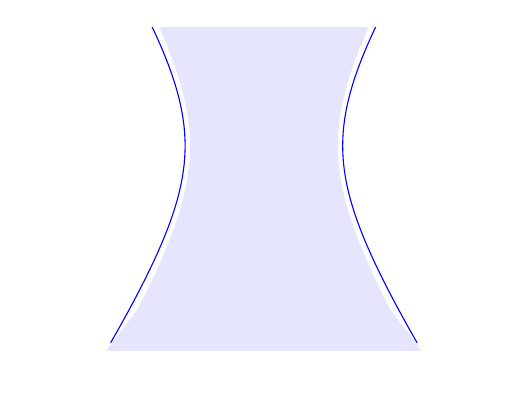
\begin{tikzpicture}[scale=0.5, font=\footnotesize, line join=round, line cap=round, >=stealth]
			\def\xmin{-6}\def\xmax{6}\def\ymin{-6}\def\ymax{3}
			\clip (\xmin,\ymin) rectangle (\xmax,\ymax);
			\path
			(0,0)coordinate (O)
			(4,-5.2) coordinate (M)
			(4,5.2) coordinate (N)
			(-4,5.2) coordinate (P)
			(-4,-5.2) coordinate (Q)
			;
			\fill[blue!10] (Q)--(M)--plot ({0.625*sqrt(\x*\x+9)},{\x})--(N)--(P)--plot ({0.625*sqrt(\x*\x+9)},{\x})--(Q);
			\fill[blue!10] (M)--(Q)--plot ({-0.625*sqrt(\x*\x+9)},{\x})--(P)--(N)--plot ({-0.625*sqrt(\x*\x+9)},{\x})--(M);
			\draw[smooth,variable=\x,blue] plot ({0.667*sqrt(\x*\x+9)},{\x});
			\draw[smooth,variable=\x,blue] plot ({-0.667*sqrt(\x*\x+9)},{\x});
		\end{tikzpicture}}
	\loigiai{Chọn hệ trục tọa độ $Oxy$ như hình vẽ.
		\begin{center}	
			\begin{tikzpicture}[scale=0.6, font=\footnotesize, line join=round, line cap=round, >=stealth]
				\def\xmin{-6}\def\xmax{6}\def\ymin{-6}\def\ymax{3}\pgfmathsetmacro\c{sqrt(13)}
				\draw[->] (\xmin-0.2,0)--(\xmax+0.2,0) node[below] {\footnotesize $x$};
				\draw[->] (0,\ymin-0.2)--(0,\ymax+1) node[right] {$y$};
				\clip (\xmin,\ymin) rectangle (\xmax,\ymax);
				\path
				(0,0)coordinate (O)
				(-2,0) coordinate (A_1)
				(2,0) coordinate (A_2)
				(-\c,0) coordinate (F_1)
				(\c,0) coordinate (F_2)
				(4,-5.2) coordinate (M)
				(4,5.2) coordinate (N)
				(-4,5.2) coordinate (P)
				(-4,-5.2) coordinate (Q)
				(0,3) coordinate (H)
				(0,-5.2) coordinate (K)
				;
				\fill[blue!10] (Q)--(M)--plot ({0.625*sqrt(\x*\x+9)},{\x})--(N)--(P)--plot ({0.625*sqrt(\x*\x+9)},{\x})--(Q);
				\fill[blue!10] (M)--(Q)--plot ({-0.625*sqrt(\x*\x+9)},{\x})--(P)--(N)--plot ({-0.625*sqrt(\x*\x+9)},{\x})--(M);
				\draw[smooth,variable=\x,blue] plot ({0.667*sqrt(\x*\x+9)},{\x});
				\draw[smooth,variable=\x,blue] plot ({-0.667*sqrt(\x*\x+9)},{\x});
				\draw (H)--(K) (A_1)--(A_2);
				\foreach \x/\g in {A_1/-40,A_2/240,O/-120,H/-30,K/-40}		\fill (\x) circle (1.5pt) ($(\x)+(\g:7mm)$) node{$\x$};
			\end{tikzpicture}
		\end{center}
	Theo giả thiết, ta có $\heva{&HK=150\\&OH=\dfrac{2}{3}OK}\Leftrightarrow \heva{&OH+OK=150\\& OH=\dfrac{2}{3}OK}\Leftrightarrow \heva{&OH=60\\&OK=90.}$\\
	Vậy $OH=60$ m và $OK=90$ m.\\
	 Gọi $\Delta_1$ là đường thẳng đi qua $H$ và vuông góc với $Oy$ tại $H$, suy ra $\Delta_1\colon y=60$.\\
		$\Delta_1$ cắt hypebol tại điểm $M$ có hoành độ dương và thỏa mãn $\dfrac{x^2}{28^2}-\dfrac{60^2}{42^2}=1$\\
		$\Rightarrow x=4\sqrt{149}\Rightarrow r_1=HM=x_M\approx 48{,}826$ m.\\
	 Gọi $\Delta_2$ là đường thẳng đi qua $K$ và vuông góc với $Oy$ tại $K$, suy ra $\Delta_2\colon y=-90$.\\
		$\Delta_2$ cắt hypebol tại điểm $N$ có hoành độ dương và thỏa mãn $\dfrac{x^2}{28^2}-\dfrac{90^2}{42^2}=1$\\
		$\Rightarrow x=4\sqrt{274}\Rightarrow r_2=KN=x_N\approx 66{,}212$ m.\\
	Vậy $T=r_1+r_2\approx 115$	m.
		}
\end{ex}

\begin{ex}%[0H9V5-0]
	Ta biết rằng mặt trăng chuyển động quanh trái đất theo quỹ đạo là một elip mà trái đất là một tiêu điểm. Elip có chiều dài trục lớn và trục nhỏ lần lượt là $769266$ (km) và $768106$ (km). Tính khoảng cách ngắn nhất từ trái đất đến mặt trăng (đơn vị $10^3$ km), biết rằng cách khoảng cách đó đạt được khi trái đất và mặt trăng nằm trên trục lớn của elip.
		\shortans{$364$}
		\begin{center}
			\begin{tikzpicture}[scale=1, font=\footnotesize, line join=round, line cap=round, >=stealth]
				\def\xmin{-3.5}\def\xmax{3.5}\def\ymin{-2.5}\def\ymax{2.5}\pgfmathsetmacro\c{1.5}
				\clip (\xmin,\ymin) rectangle (\xmax,\ymax);
				\path
				(-\c,0) coordinate (F_1)
				(1.5,1.6) coordinate (M)
				;
				\draw [blue]
				(0,0)  ellipse (2.5cm and 2cm);
				\fill[blue] (M)node[above right ]{Mặt trăng} circle (2.5pt);
				\fill[cyan] (F_1)  node[below]{Trái đất} circle (5pt);
			\end{tikzpicture}
		\end{center}
\loigiai{
	Phương trình chính tắc của elip có dạng là $\dfrac{x^2}{a^2}+\dfrac{y^2}{b^2}=1\  (a>b>0)$.\\
	Elip có độ dài trục lớn $2a=769266\Leftrightarrow a=384633$;\\
	Elip có độ dài trục bé $2b=768106\Leftrightarrow b=384053$.\\
	Ta có $c=\sqrt{a^2-b^2}\approx 21115$.\\
	Vậy  khoảng cách ngắn nhất từ trái đất đến mặt trăng là $a-c=363518\approx 364\cdot 10^3$ (km).}
\end{ex}

\begin{ex}%[0H9H5-3]
	Cho phương trình chính tắc của elip $(E)\colon \dfrac{x^2}{a^2}+\dfrac{y^2}{b^2}=1$, ($a,b>0$). Biết elip có hai đỉnh trên trục nhỏ cùng với hai tiêu điểm tạo thành một hình vuông có diện tích bằng $32$. Hãy tính $T=2a+b^2$?
		\shortans{$16$}
	\loigiai{
	\immini{
	Phương trình chính tắc của elip $(E)\colon \dfrac{x^2}{a^2}+\dfrac{y^2}{b^2}=1$, ($a>b>0$) và $c^2=a^2-b^2$.\\
	Hai đỉnh trên trục nhỏ $B_1(0;-b)$, $B_2(0;b)$ và hai tiêu cự $F_1(-c;0)$, $F_2(c;0)$ là bốn đỉnh của một hình vuông nên $b=c$.\\
	Mặt khác, diện tích hình vuông bằng $32$ nên\\
	 $2c\cdot 2b=32\Rightarrow b^2=8$.\\
	Vậy $b=c=8$ và $a^2=b^2+c^2=16\Rightarrow a=4$.}	{\begin{tikzpicture}[scale=1, font=\footnotesize, line join=round, line cap=round, >=stealth]
			\def\xmin{-2.5}\def\xmax{2.5}\def\ymin{-2}\def\ymax{2}\pgfmathsetmacro\c{1.4}
			\draw[->] (\xmin-0.2,0)--(\xmax+0.2,0) node[below] {\footnotesize $x$};
			\draw[->] (0,\ymin-0.2)--(0,\ymax+0.2) node[right] {$y$};
			\draw (0,0) node [below left] {$O$};
			\clip (\xmin,\ymin) rectangle (\xmax,\ymax);
			\path
			(-2,0) coordinate (A_1)
			(2,0) coordinate (A_2)
			(0,-1.4) coordinate (B_1)
			(0,1.4) coordinate (B_2)
			(-\c,0) coordinate (F_1)
			(\c,0) coordinate (F_2)
			;
			\draw [blue]
			(0,0)  ellipse (2cm and 1.4cm);
			\draw
			(B_1)--(F_1)--(B_2)--(F_2)--cycle
			;
			\foreach \x/\g in {F_1/-90,F_2/-90,B_1/-50,B_2/50}
			\fill (\x) circle (1.5pt) ($(\x)+(\g:3mm)$) node{$\x$};
		\end{tikzpicture}	}
		Phương trình chính tắc của elip là $\dfrac{x^2}{16}+\dfrac{y^2}{8}=1$ và $T=2a+b^2=2\cdot 4+(2\sqrt{2})^2=16$.
	}	
\end{ex}


\begin{ex}%[0H9V5-0]
	Để cắt một bảng hiệu quảng cáo hình elip có trục lớn bằng $80$ cm và trục nhỏ bẳng $40$ cm từ một tấm ván ép hình chữ nhật $ABCD$ có kích thước $80$ cm $40$ cm. Người ta vẽ hình elip đó lên tấm ván ép (như hình vẽ) bằng một vòng dây qua hai cái đinh ghim vào hai tiêu điểm. Hỏi phải lấy vòng dây có độ dài là bao nhiêu cm (làm tròn đến hàng đơn vị).
	\shortans{$175$}
	\begin{center}
		\begin{tikzpicture}[scale=0.7, font=\footnotesize, line join=round, line cap=round, >=stealth]
			\def\xmin{-5}\def\xmax{5}\def\ymin{-3}\def\ymax{3}\pgfmathsetmacro\c{2*sqrt(3)}
			\draw[->] (\xmin-0.2,0)--(\xmax+0.2,0) node[below] {\footnotesize $x$};
			\draw[->] (0,\ymin-0.2)--(0,\ymax+0.2) node[right] {$y$};
			\draw (0,0) node [below left] {$O$};
			\clip (\xmin,\ymin) rectangle (\xmax,\ymax);
			\path
			(-4,0) coordinate (A_1)node[below left]{$-a$}
			(4,0) coordinate (A_2)node[below right]{$a$}
			(0,-2) coordinate (B_1)node[below left]{$-b$}
			(0,2) coordinate (B_2)node[above left]{$b$}
			(-\c,0) coordinate (F_1)node[above]{$-c$}
			(\c,0) coordinate (F_2)node[above left]{$c$}
			(3,1.32) coordinate (M)
			(-4,2) coordinate (A)
			(-4,-2) coordinate (D)
			(4,2) coordinate (B)
			(4,-2) coordinate (C)
			;
			\draw 
			(0,0)  ellipse (4cm and 2cm)
			(A)--(B)--(C)--(D)--(A) (F_1)--(M)--(F_2)--cycle
			;
			\fill (M)node[above]{$M$} circle (1.5pt);
			\foreach \x/\g in {F_1/-90,F_2/-90,A/135,B/45,C/-45,D/-135}
			\fill (\x) circle (1.5pt) ($(\x)+(\g:4mm)$) node{$\x$};
		\end{tikzpicture}
	\end{center}
	\loigiai{ 
		Ta có $\heva{&2a=80\\& 2b=40}\Leftrightarrow \heva{&a=40\\&b=20.}$
		Khi đó $c=\sqrt{a^2-b^2}=20\sqrt{3}$.
		\begin{itemize}
			\item Tiêu điểm $F_1(-20\sqrt{3};0)$ và $F_2(20\sqrt{3};0)$. Do đó hai đinh cách mép tấm ván là $F_1A_1=F_2A_2=40-20\sqrt{3}\approx 5{,}36$ cm.
			\item Đỉnh $B_2(0;40)$.
			\item $MF_1=\sqrt{(20\sqrt{3})^2+40^2}=20\sqrt{7}$ cm.
			\item Vòng dây có độ dài $F_1F_2+MF_1+MF_2=40\sqrt{3}+40\sqrt{7}\approx 175$ cm.
		\end{itemize}
	}	
\end{ex}
\Closesolutionfile{ans}
\indapan{6}{ans/ans-0-C7B4.D2-KQ}
